\newpage

\section{\MakeUppercase{Cross-Border Payments in the Real World}}\label{sec:payments}

%\subsection*{Abstract}

\subsection{Introduction}

Now, let us analyze a typical cross-border transaction in which a local producer imports some goods from abroad and commits to paying a foreign counterparty. Again, let us use the case of cross-border trade transaction between two business units of the United States and Mexico such as in \citep[p.~500-501]{lavoie2022}, but not exactly following that exposition. In terms of money of account, the transacting counterparties have many options, of which there are two main ones. They can use either the U.S. dollar or the Mexican peso. Then, let us assume that they agree on the former. 

With all the assumptions made above, there are two typical cases: (1) a U.S. resident makes imports paid in the U.S. dollar via a local bank. Generally, this is the case of imports paid in \textit{domestic} money. And (2) a Mexico resident makes imports paid in the U.S. dollar via a local bank. Generally, this is the case of imports paid in \textit{foreign} money.

It is resonable to claim that just-mentioned counterparties might decide on the money of account of a third country, for example, British pound (\pounds), Chinese yuan or other. Nevertheless, analyically such an option is not a distinctive from the previous two. It falls into the category of the payments in foreign money with more complexity being added on. That is why it is not considered here in detail.

The next subsections, \ref{sec:xpay_dom} and \ref{sec:xpay_frn}, below consider these two cases through the framework developed above that money is a system of debt-credit relationships. For simplicity we consider imports, while the same logic applies to all other cases of payments made cross-border such as financial investments.

As a side note, during discussion of the monetary side of international trade, \cite{ehnts2024} observes: ``Imports thus lead to additional income abroad, and thus purchasing power is \textit{lost} for the domestic monetary circuit.''~\citep[p.~68, emhasis added]{ehnts2024} 

This paper suggests an analytical framework to test such a hypothesis in terms of the lost purchasing power during imports or other purchases abroad such as of financial securities. Note that the above statement (i) assumes an already existing purchasing power in the hands of a domestic individual or producer, and (ii) is neutral to the money of account in which payments for imports were made. In other words, whatever money of account---domestic or foreign---is relied upon for cross-border payments, there is a general outcome of lost purchasing power for the domestic monetary circuit. By standard definition, purchasing power is a positive balance on an individual or producer's checking (current) account with a local bank, and the domestic monetary circuit consists of all units, such as governing authorities, banks, producers, and individuals, which are residents of a country. 

One might suggest that purchasing power means it can be nonexistance right now but endogenuously created on demand by a bank. To address this extended meaning of purchasing power this paper considers two cases for each subsection that follows: (i) endogenous creation of money and (ii) pre-existing money.

\subsection{\textit{Domestic} Money of Account}\label{sec:xpay_dom}

Given the exposition in Figure~\ref{fig:minsky_scheme}, on p.~\pageref{fig:minsky_scheme}, featuring United States and Italy, consider a hypothetical cross-border transaction between two businesses n the U.S. and Mexico. In this transaction, there are two counterparties: a U.S.-based firm $B$ and a Mexican-based firm $C$. The former is an importer and the latter is an exporter of the products made in Mexico. Upon mutual agreement, the payment is to be undertaken in the U.S. dollars. 

As shown in Figure~\ref{fig:minsky_scheme}, there is an underlying assumption that both firms are customers of their domestic banks. The U.S.-based firm is a customer of the U.S.-based bank $R_2$, which is a member bank of the Federal Reserve system and hence it has a reserve accout with the New York Federal Reserve Bank for payments in the U.S. dollar (USD). The Mexico-based firm is a customer of the local commercial bank $R_1$, which is supervised by the Mexico's central bank and hence has a reserve account with the latter for payments in Mexican peso (MXN). However, the same Mexico-based commercial bank $R_1$ has a correspondent banking relationship with the U.S.-based bank $R_2$ just mentioned. Under such a relationship these banks agree to carry out payments either in USD or MXN if their customers decide a particular money of account for transactions. However, Figure~\ref{fig:minsky_intl} shows \textit{only} a correspondent relationship between banks $R_2$ and $R_1$ for payments in U.S. dollar. It means that the U.S.-based bank $R_2$ is on the debt side and the Mexico-based bank $R_1$ is on the creditor side of the debt-credit relationship due today continuously, which is denominated in the U.S. dollar. Note that if the firms were to decide that payment is in Mexican peso, then the commercial banks of two countries would have used the correspondent bank account denominated in Mexican peso and their positions swapped: the U.S.-based bank $R_2$ is on the credit side and the Mexico-based bank is on the debt side.

\subsubsection{Endogenous Money}

Let us now proceed to the payment itself. In order to provide a full exposition of endogenous money, another assumption is that the U.S.-based firm $B$, the payer or payment initiator, has a zero balance on its checking account with bank $R_2$. Hence, $B$ borrows from $R_2$ a required sum of US dollars to be immediately paid in favor of the Mexico-based firm $C$, the payee or payment beneficiary. This is a triangle between the counterparties of the payment that was shown ealier in Figure~\ref{fig:bank_mk_loan} on p.~\pageref{fig:bank_mk_loan}. However, because there is no direct relationship between the U.S.-based bank and the Mexico-based firm $C$, it is the Mexico-based bank $R_1$ that stands between them. Hence, Figure~\ref{fig:bank_mk_loan} must be re-drawn in the following way, see Figure~\ref{fig:US_MX_payment1} below. 

\begin{figure}[!ht]
\centering
\vspace{.1in}
\captionsetup{width=1\linewidth,labelfont=bf}
\usetikzlibrary {matrix}
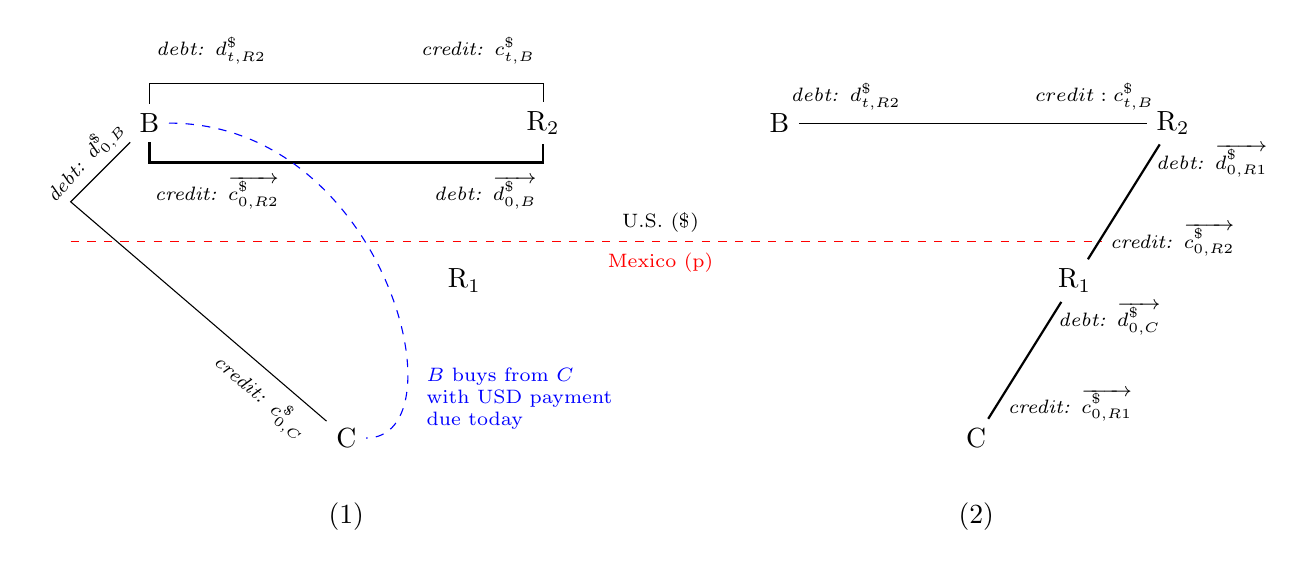
\begin{tikzpicture}
  \draw[help lines,white] (0,0) grid (15,5);
  % Left-hand side part of the Figure
  \node         (B)         at (1,4.5) {B};
  \node         (R2)        at (6,4.5) {R$_2$};
  \node         (R1)        at (5,2.5) {R$_1$};
  \node         (C)         at (3.5,0.5) {C};
  \node                     at (3.5,-.5) {(1)};
  \draw[red,dashed] (0,3) -- (13.1,3); 
  \node[black] at (7.5,3.2) {\textsuperscript{U.S. (\$)}};
  \node[red] at (7.5,2.7) {\textsuperscript{Mexico (p)}};
  \draw[black] (B.north) |- (4,5) -| (R2.north);
  \draw[black,thick] (B.south) |- (4,4) -| (R2.south);
  \node at (3.5,5.4) {\textsuperscript{\textit{debt: }$d^{\$}_{t,R2}$ \hspace{.7in} \textit{credit: }$c^{\$}_{t,B}$}};
  \node at (3.5,3.6) {\textsuperscript{\textit{credit: }$\overrightarrow{c^{\$}_{0,R2}}$ \hspace{.7in} \textit{debt: }$\overrightarrow{d^{\$}_{0,B}}$}};  
  \draw[dashed,blue] (B) .. controls +(left:-3cm) and +(left:-1.5cm) .. (C);
  \node[blue,align=left,font=\scriptsize] at (5.7,1) {$B$ buys from $C$\\with USD payment\\due today};
  \draw (B) -- (0,3.5) -- (C); 
  \node[rotate=49] at (.2,4) {\textsuperscript{\textit{debt: }$d^{\$}_{0,B}$}};
  \node[rotate=-40] at (2.4,1) {\textsuperscript{\textit{credit: }$c^{\$}_{0,C}$}};
  % Right-hand side part of the Figure
  \node         (B)         at (9,4.5) {B};
  \node         (R2)        at (14,4.5) {R$_2$};
  \node         (R1)        at (12.75,2.5) {R$_1$};
  \node         (C)         at (11.5,0.5) {C};
  \node                     at (11.5,-.5) {(2)};
  \draw (B) -- (R2) node[midway,sloped,above]%
        {\textsuperscript{\textit{debt: }$d^{\$}_{t,R2}$ \hspace{.6in} $credit: c^{\$}_{t,B}$}};
  \draw[thick] (C) -- (R1); \draw[thick] (R1) -- (R2);
  \node at (14.5,4) {\textsuperscript{\textit{debt: }$\overrightarrow{d^{\$}_{0,R1}}$}};
  \node at (14,3) {\textsuperscript{\textit{credit: }$\overrightarrow{c^{\$}_{0,R2}}$}};
  \node at (13.2,2) {\textsuperscript{\textit{debt: }$\overrightarrow{d^{\$}_{0,C}}$}};
  \node at (12.7,.9)   {\textsuperscript{\textit{credit: }$\overrightarrow{c^{\$}_{0,R1}}$}};
  %\draw[thick] (C) -- (R2) node[midway,sloped,below]%
  %      {\textsuperscript{$credit: \overrightarrow{c^{\$}_{0,R}}$ \hspace{.45in} $debt: \overrightarrow{d^{\$}_{0,B}}$}};
\end{tikzpicture}
\caption{A U.S.-based bank $R_2$ provides U.S.-based firm $B$ with a loan in US dollars for $B$'s immediate payment to the Mexico-based firm $C$, which is customer of Mexico-based bank $R_1$}%
\label{fig:US_MX_payment1}
\vspace{.1in}
\end{figure}

Note the debt and credit positions of the counterparties after the payment was completed on right-hand side of the figure. In particular, the U.S.-based bank $R_2$ retained its debt position $\overrightarrow{d^{\$}_0}$ after it was endogenously created against U.S.-based firm $B$, but now it is against a Mexico-based bank $R_1$. Overall, the cross-border payment is a creation of debt-credit relationships of due today continuously.

\subsubsection{Pre-Existing Money}

If one takes a view that a U.S.-based $B$ has already a U.S. dollar balance with its U.S.-based bank $R_2$ enough to make a payment to the Mexico-based firm $C$, then its exposition is simplier than in the previous situation. See Figure~\ref{fig:US_MX_payment2}, below on p.~\pageref{fig:US_MX_payment2}. Thanks to its credit ($\overrightarrow{c^{\$}_{0}}$) position on its bank, $B$ just provides the latter with a pyamnet order to the beneficiary of $C$. Again, thanks to the established correspondent banking relationship between $R_2$ and a Mexico-based bank $R_1$, then $R_2$ acts upon its already existing debt-credit relationship, where it has a debt position ($\overrightarrow{d^{\$}_{0}}$), and re-assign the credit position from $B$ to $R_1$. It also instructs $R_1$ to credit $C$'s U.S. dollar account for the payment's value. In effect, $R_1$ and $C$ create new debt-credit relationship due today contonuously, which is denominated in the U.S. dollar. Once, this is done the U.S. dollar payment is compelte.

Note again that a U.S.-based bank $R_2$ does not lose its debt position ($\overrightarrow{d^{\$}_{0}}$) because of the payment. Instead, it just re-assigned its counterparty from a U.S.-based firm $B$ to a Mexico-based correspondent bank $R_1$. The size of the balance sheet of $R_2$ did not shrink. Bank money in terms of their size did not change at the moment when the payment was complete.

\begin{figure}[!ht]
\centering
\vspace{.1in}
\captionsetup{width=1\linewidth,labelfont=bf}
\usetikzlibrary {matrix}
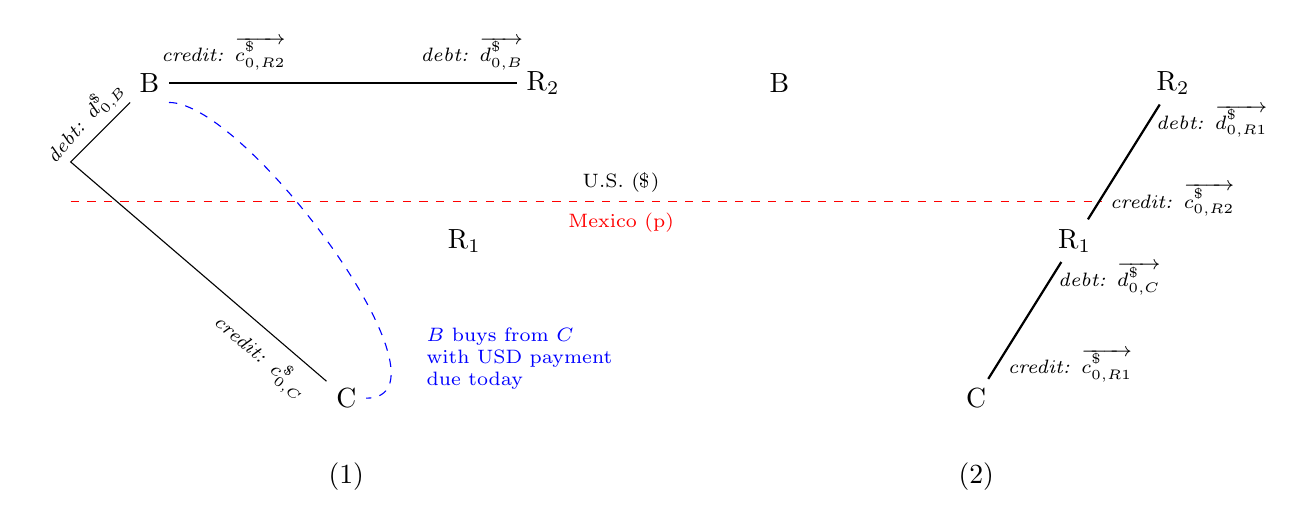
\begin{tikzpicture}
  \draw[help lines,white] (0,0) grid (15,5);
  % Left-hand side part of the Figure
  \node         (B)         at (1,4.5) {B};
  \node         (R2)        at (6,4.5) {R$_2$};
  \node         (R1)        at (5,2.5) {R$_1$};
  \node         (C)         at (3.5,0.5) {C};
  \node                     at (3.5,-.5) {(1)};
  \draw[red,dashed] (0,3) -- (13.1,3); 
  \node[black] at (7,3.2) {\textsuperscript{U.S. (\$)}};
  \node[red] at (7,2.7) {\textsuperscript{Mexico (p)}};
  %\draw[black] (B.north) |- (4,5) -| (R2.north);
  %\draw[black,thick] (B.south) |- (4,4) -| (R2.south);
  \draw[thick] (B) -- (R2) node[midway,sloped,above] {\textsuperscript{\textit{credit: }$\overrightarrow{c^{\$}_{0,R2}}$ \hspace{.6in} \textit{debt: }$\overrightarrow{d^{\$}_{0,B}}$}};
  %\node at (3.5,5.4) {\textsuperscript{\textit{debt: }$d^{\$}_{t,R2}$ \hspace{.7in} \textit{credit: }$c^{\$}_{t,B}$}};
  %\node at (3.5,3.6) {\textsuperscript{\textit{credit: }$\overrightarrow{c^{\$}_{0,R2}}$ \hspace{.7in} \textit{debt: }$\overrightarrow{d^{\$}_{0,B}}$}};  
  \draw[dashed,blue] (B.south east) .. controls +(left:-1cm) and +(left:-1.5cm) .. (C);
  \node[blue,align=left,font=\scriptsize] at (5.7,1) {$B$ buys from $C$\\with USD payment\\due today};
  \draw (B) -- (0,3.5) -- (C); 
  \node[rotate=49] at (.2,4) {\textsuperscript{\textit{debt: }$d^{\$}_{0,B}$}};
  \node[rotate=-40] at (2.4,1) {\textsuperscript{\textit{credit: }$c^{\$}_{0,C}$}};
  % Right-hand side part of the Figure
  \node         (B)         at (9,4.5) {B};
  \node         (R2)        at (14,4.5) {R$_2$};
  \node         (R1)        at (12.75,2.5) {R$_1$};
  \node         (C)         at (11.5,0.5) {C};
  \node                     at (11.5,-.5) {(2)};
  %\draw (B) -- (R2) node[midway,sloped,above]%
  %      {\textsuperscript{\textit{debt: }$d^{\$}_{t,R2}$ \hspace{.6in} $credit: c^{\$}_{t,B}$}};
  \draw[thick] (C) -- (R1); \draw[thick] (R1) -- (R2);
  \node at (14.5,4) {\textsuperscript{\textit{debt: }$\overrightarrow{d^{\$}_{0,R1}}$}};
  \node at (14,3) {\textsuperscript{\textit{credit: }$\overrightarrow{c^{\$}_{0,R2}}$}};
  \node at (13.2,2) {\textsuperscript{\textit{debt: }$\overrightarrow{d^{\$}_{0,C}}$}};
  \node at (12.7,.9)   {\textsuperscript{\textit{credit: }$\overrightarrow{c^{\$}_{0,R1}}$}};
\end{tikzpicture}
\caption{A U.S.-based bank $R_2$ provides U.S.-based firm $B$ with a loan in US dollars for $B$'s immediate payment to the Mexico-based firm $C$, which is customer of Mexico-based bank $R_1$}%
\label{fig:US_MX_payment2}
\vspace{.1in}
\end{figure}

Both expositions, in Figures~\ref{fig:US_MX_payment1} and \ref{fig:US_MX_payment2}, explain in detail what a senior official of the Inernational Monetary Fund (IMF)\footnote{Tobias Adrian, the Financial Councellor and Director of the Monetary and Capital Markets Department of the IMF. See \url{https://www.imf.org/en/About/senior-officials/Bios/tobias-adrian}} was talking about the essencial elements of cross-border payments. He used rather obscure language while talking in breif on the subject:

\begin{quote}
When a Moroccan ceramics business exports dinnerware to nearby Spain, it receives
money in its account through a complex web of inter-linkages between banks, possibly
going through Paris and New York. The payment is routed through banks
that know and trust each other. Money \textit{does not really change hands}; instead, \textit{each
bank offers credit to the next one in line}. As a result, the small Moroccan business
may face delays in receiving money and will pay high fees, hurting its bottom line.
\citep[emphasis added]{adrian2023}
\end{quote}

In his commentary \citeauthor{adrian2023} surely tended to sound as an orthodox economist, for whom ``money'' is both a tangable cash, which every indiviual has an experience of, and intangable reserves or settlement balances, which every commercial bank use today at its account with a central bank. His usage of word ``credit'' intended to be orthodox, too, in the meaning of ``loan.'' However, it is rather not. Instead, \citeauthor{adrian2023}'s ``credit'' has the meaning this paper is conceptualizing: $\overrightarrow{c_0}$. In the described case of a Moroccan ceramics producer, the only credit that ``each bank offers \dots to the next one in line'' is the one that is part of debt-credit relationships due today continuously. Indeed, it might be the case that in Morocco local banks do not have direct correspondent relationships with banks located in the countries from which foreign purchases of Moroccan ceramics originate. Hence, their correspondent banking relationships might be done via those large banks, based in major global financial centers such as New York, London, Paris and others, that serve as specialists in correspondent banking business. As shown in Figures~\ref{fig:US_MX_payment1} and \ref{fig:US_MX_payment2}, there is a short line of two banks, where $R_2$ provides $R_1$ with a debt-credit relationship in which they have respectively debt ($\overrightarrow{d^{\$}_0}$) and credit ($\overrightarrow{c^{\$}_0}$) positions. Whereas in the \citeauthor{adrian2023}'s example that line is longer by, at least, one more bank, being based in Paris or New York. And these banks create new debt-credit relationships between each other by the same principle.

\subsection{\textit{Foreign} Money of Account}\label{sec:xpay_frn}

Now, let us consider the reverse situation, when a Mexico-based firm $C$ from Figure~\ref{fig:minsky_intl}, p~\pageref{fig:minsky_intl}, requires a payment in U.S. dollars to be made in favor of the U.S.-based firm $B$. In other words, the payer uses foreign money of account in order to complete its payment committed.

The next two subsections consider two starting conditions: (i) endogenous money upproach, when basic assumption is that all unit have zero balances on its reserve or checking accounts, and (ii) pre-existing money. 

\subsubsection{Endogenous Money}

Under endogenous money approach the following transactions take place. Since firm $C$ has zero U.S. dollar and Mexican peso balances on its checking accounts with the Mexico-based bank, then it asks the latter to provide a loan either in Mexican pesos or in U.S. dollars. Under high level of financial liberalization, the Mexico's transacting counterparties are free to decide which money of account to use. Considerations of interest rate and borrower's ability to access credits in that money of account on the due date will be taking into account while making final decision. Let's assume they agree on the loan in the U.S. dollar. Then, a cerain chain of actions with debt-credit relationships will place as shown in Figure~\ref{fig:US_MX_payment3} below, p.~\pageref{fig:US_MX_payment3}. Such a chain includes creations, reuses and set-offs of the DCRs. The left-hand side part of the figure depicts initiation of the payment: (i)~since $C$ buys from $B$ they become debtor and creditor, respecively; (ii)~to make a U.S. dollar payment $C$ borrows from its bank $R_1$ for a period of, for example, three months ($t=90$ days), (iii)~while the latter borrows overnight from $R_2$ ($t=1$ day) to accomodate its customer. As a result, five new debt-credit relationships were created. Then, the payment by $C$ to $B$ is handled as a series of set offs and reuse of just created DCRs: (i) for $C$ its $d^{\$}_{0,C}$ is set off with $\overrightarrow{c^{\$}_{0,R1}}$, (ii) for $R_1$ its $\overrightarrow{d^{\$}_{0,C}}$ is set off with $\overrightarrow{c^{\$}_{0,R2}}$, and (iii) for $R_2$, acting by the order from $R_1$, reuses its formerly $\overrightarrow{d^{\$}_{0,R1}}$ to currently $\overrightarrow{d^{\$}_{0,B}}$. Lastly, the right-hand side of Figure~\ref{fig:US_MX_payment3} shows the moment, when payment is completed and all the discussed counterparties have certain debt or credit positions. 

\begin{figure}[!ht]
\centering
\vspace{.1in}
\captionsetup{width=1\linewidth,labelfont=bf}
\usetikzlibrary {matrix}
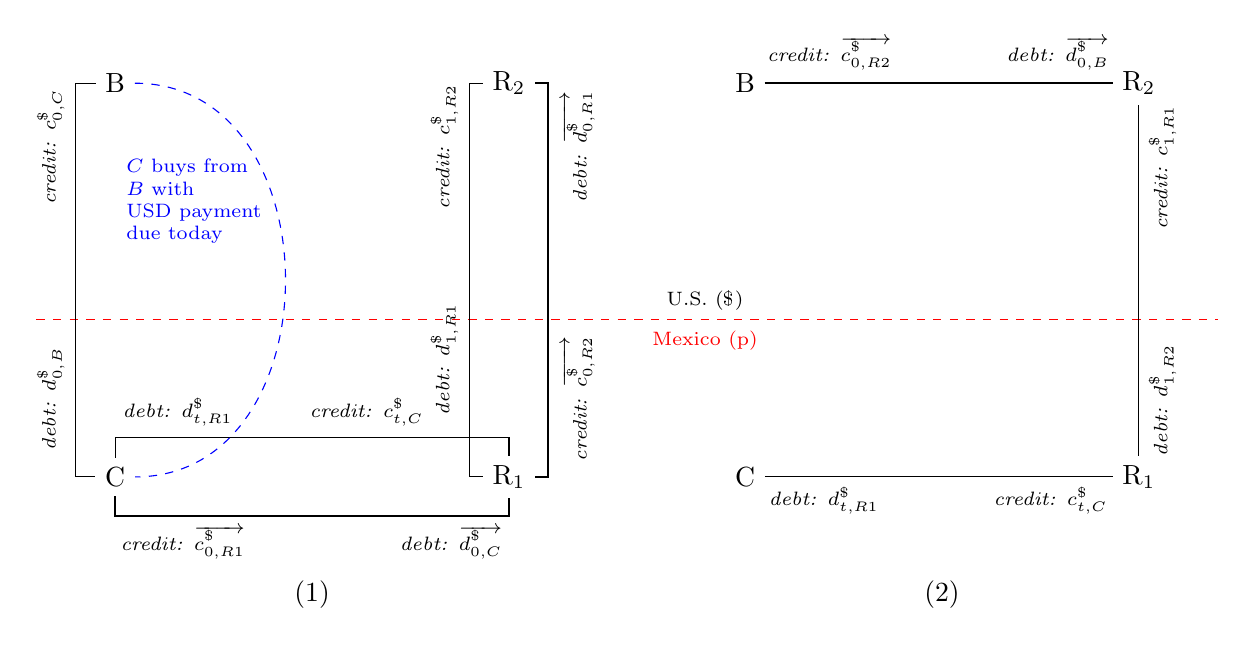
\begin{tikzpicture}
  \draw[help lines,white] (0,0) grid (15,6);
  % Left-hand side part of the Figure
  \node         (B)         at (1,6) {B};
  \node         (R2)        at (6,6) {R$_2$};
  \node         (R1)        at (6,1) {R$_1$};
  \node         (C)         at (1,1) {C};
  \node                     at (3.5,-0.5) {(1)};
  \draw[red,dashed] (0,3) -- (15,3); 
  \node[black] at (8.5,3.2) {\textsuperscript{U.S. (\$)}};
  \node[red] at (8.5,2.7) {\textsuperscript{Mexico (p)}};
  %\draw[red,dashed] (0,3.5) -- (15,3.5); 
  %\node[red] at (8.5,3.7) {\textsuperscript{United States, \$}};
  %\node[red] at (8.5,3.2) {\textsuperscript{Mexico, peso}};
  \draw[black]   (C.north) |- (4,1.5) -| (R1.north);
  \draw[black,thick]   (C.south) |- (4,0.5) -| (R1.south);
  \node at (1.8,1.8) {\textsuperscript{\textit{debt: }$d^{\$}_{t,R1}$}};
  \node at (4.2,1.8) {\textsuperscript{\textit{credit: }$c^{\$}_{t,C}$}};
  %\node at (3.5,1.7) {\textsuperscript{\textit{debt: }$d^{\$}_{t,R1}$ \hspace{.7in} \textit{credit: }$c^{\$}_{t,C}$}};
  \node at (3.5,0.15) {\textsuperscript{\textit{credit: }$\overrightarrow{c^{\$}_{0,R1}}$ \hspace{.7in} \textit{debt: }$\overrightarrow{d^{\$}_{0,C}}$}};  
  \draw[dashed,blue] (B) .. controls +(left:-2.8cm) and +(left:-2.8cm) .. (C);
  \node[blue,align=left,font=\scriptsize] at (2,4.5) {$C$ buys from\\$B$ with\\USD payment\\due today};
  \draw (B) -| (.5,3) |- (C);
  \node[rotate=90] at (0.2,5.2) {\textsuperscript{\textit{credit: }$c^{\$}_{0,C}$}};
  \node[rotate=90] at (0.2,2.0) {\textsuperscript{\textit{debt: }$d^{\$}_{0,B}$}};
  \draw[thin]  (R1) -| (5.5,3) |- (R2);
  \node[rotate=90] at (5.2,5.2) {\textsuperscript{\textit{credit: }$c^{\$}_{1,R2}$}};
  \node[rotate=90] at (5.2,2.5) {\textsuperscript{\textit{debt: }$d^{\$}_{1,R1}$}};
  \draw[thick] (R1) -| (6.5,3) |- (R2);
  \node[rotate=90] at (6.9,5.2) {\textsuperscript{\textit{debt: }$\overrightarrow{d^{\$}_{0,R1}}$}};
  \node[rotate=90] at (6.9,2.0) {\textsuperscript{\textit{credit: }$\overrightarrow{c^{\$}_{0,R2}}$}};
  % Right-hand side part of the Figure
  \node         (B)         at (9, 6) {B};
  \node         (R2)        at (14,6) {R$_2$};
  \node         (R1)        at (14,1) {R$_1$};
  \node         (C)         at (9, 1) {C};
  \node                     at (11.5,-0.5) {(2)};
  \draw[thick] (B) -- (R2) node[midway,sloped,above]%
        {\textsuperscript{\textit{credit: }$\overrightarrow{c^{\$}_{0,R2}}$ \hspace{.5in} \textit{debt: }$\overrightarrow{d^{\$}_{0,B}}$}};
  \draw[thin] (C) -- (R1)  node[midway,sloped,below]%
        {\textsuperscript{\textit{debt: }${d^{\$}_{t,R1}}$ \hspace{.5in} \textit{credit: }${c^{\$}_{t,C}}$}}; 
  \draw[thin] (R1) -- (R2) node[midway,sloped,below]%
        {\textsuperscript{\textit{debt: }${d^{\$}_{1,R2}}$ \hspace{.5in} \textit{credit: }${c^{\$}_{1,R1}}$}};
\end{tikzpicture}
\caption{(1) a U.S. dollar payment by $C$ to $B$ is initiated as $C$ borrows from $R_1$, and the latter borrows overnight ($t=1$) from $R_2$, and (2) the payment is completed}%
\label{fig:US_MX_payment3}
\vspace{.1in}
\end{figure}

Note the positions of the counterparties involved to facilitate the payment: both of the Mexico-based units---firm $C$ and bank $R_1$---have \textit{dated} debt-credit relationships. One of them is with each other. Second is between $R_1$ and the U.S.-based $R_2$. Lastly, the U.S.-based units---firm $B$ and bank $R_2$ have a debt-credit relationship due today continuously. Effectively, the U.S. dollar payment has been facilitated by the U.S.-bank, which expanded its balance sheet via, first, providing a U.S. dollar loan to the Mexico-based bank. Via a loan, it created two debt-credit relationships (DCRs) with a Mexican bank: one dated and another is due today continuously. Then, on the latter's order, it re-assigned the credit position within the second DCR from the Mexican bank to the U.S.-based firm $B$. This endouguous creation of money for the U.S. dollar payment, as described, does not reveal a loss of purchasing power.   

This exposition differs from the one in \cite{lavoie2014,lavoie2022}, see section 7.1.3 'A Transaction Initiated by the Banking Sector' of this book present in both 1st and 2nd editions. The latter provides an endogenous money example for a cross-border transaction between Mexico and the United States. \citeauthor{lavoie2022} starts off with a Mexican bank called Banamex turning to a U.S. bank called City Bank for a loan denominated in U.S. dollar. Then, the exposition proceeds to possible reasons why Banamex acts this way:  ``We may then presume that Banamex agrees to take in the loan because it knows that some Mexican residents would like to borrow US dollars. The newly created dollars are now held by the Mexican residents. This is shown in [Table 7.2,] row 2.''~\citep[p.~501]{lavoie2022} The author explicitly resognizes those individuals that are to borrow dollars from Banamex as ``Mexican residents.'' However, Table 7.2 locates the ``newly created dollars'' as liability of City Bank, not of Banamex as endogenuous money approach postulates. It leaves a reader without due explanation why this happened. It must be explained because each commercial bank today, following domestic central bank regulation, adheres to a quite strict KYC (know your customer) policy. KYC is an internationally recognized business practice in domestic and international banking~\citep{bis2020_}. It is quite costly for a resident of one country to have bank accounts in the domestic bank as well as in the foreign bank. This situation is possible, but it is rather an exception from a more general case: residents of country have checking (current) accounts with domestic banks and their denomination is in the domestic as well as in foreign monies of account. But even if a Mexican resident had accounts at both a Mexican bank or a U.S. bank, it would choose the bank to borrow in U.S. dollars from which charges less in term of the interest rate. And then it would ask that bank to proceed with a U.S. payment. From a perspective of debt-credit relationship this paper advocates, such an exposition with unexplained shortcuts confuses rather than illuminates the reader.

\subsubsection{Pre-Existing Money}

If the same case is reconsidered by switching from endogenuous money creation to pre-existing ``purchasing power'' on the checking account of the Mexico's importer $C$, then the following exposition is proposed. 

To illustrate this case in full, in an extended form, it must be assumed that Mexico-based firm $C$ has that purchasing power on its Mexican peso checking account with a local bank $R_1$. This assumption is quite reasonable for the country which has its own money of account -- Mexican peso. How then $C$ acquires the U.S. dollars? There are several options, however, let us make another assumption of pre-existing purchasing power in U.S. dollar: there is another Mexico-based firm $D$, which is an exporter and has just been paid in the U.S. dollar thanks to prior sale of own produce. Consider this assumption as an end point of the case shown in Figures~\ref{fig:US_MX_payment1} and \ref{fig:US_MX_payment2}, above. These two prior assumptions are shown on~\pageref{fig:US_MX_payment4} in Figure~\ref{fig:US_MX_payment4}, section (1), as red and black thick lines, respectively. The former line is between $C$ and $R_1$, representing a debt-credit relationship due today continuously in Mexican peso. The latter line is beetween $D$ and $R_3$ representing similar reltionship in U.S. dollar, but it also extends to the same relationship between $R_3$ and its U.S.-based correspondent bank $R_2$, because that prior U.S. dollar payment has just happened. 

Note: two relationships between $D$---$R_3$ and $R_3$---$R_2$, in section (1) of Figure~\ref{fig:US_MX_payment4}, exist together at the very moment of the U.S. payment to $D$ is made as shown in section (2) of either Figure~\ref{fig:US_MX_payment1} or Figure~\ref{fig:US_MX_payment2}. If, for example, next moment, or day, $D$ stays idle with its U.S. dollar balance with $R_3$, the latter most likely does not with its own U.S. dollar balance with $R_2$, because it has numeruous customers requiring a U.S. dollar payment such as shown in Figure~\ref{fig:US_MX_payment3}.

Indeed, section (1) of Figure~\ref{fig:US_MX_payment4} is a starting point of the exposition of the U.S. dollar paymnet by $C$ to $B$. 

\begin{figure}[!ht]
\centering
%\vspace{.1in}
\captionsetup{width=1\linewidth,labelfont=bf}
\usetikzlibrary {matrix}
%% SECTION #1
\begin{tikzpicture}[scale=1]
  \draw[help lines,white] (0,0) grid (15,6);
  % Left-hand side part of the Figure
  \node         (B)         at (0,6) {B};
  \node         (R2)        at (7.5,6) {R$_2$};
  \node         (R1)        at (5,1) {R$_1$};
  \node         (R3)        at (10,1) {R$_3$};
  \node         (C)         at (0,1) {C};
  \node         (D)         at (15,1) {D};
  \node                     at (7.5,-0.5) {(1)};
  \node                     at (7.5,-3) {}; % blank line, separator
  \draw[black,dashed] (-.25,3.5) -- (15.25,3.5); 
  \node[black] at (13.5,3.7) {\textsuperscript{U.S. (\$)}};
  \node[red] at (13.5,3.3) {\textsuperscript{Mexico (p)}};
  %\draw[gray,dashdotted] (R1) -- (R2); \draw[gray,dashdotted] (R1) -- (R3);
  %\draw[black,dashed]  (-.25,3.55) -- (15.25,3.55); 
  %\draw[red,dashed] (-.25,3.45) -- (15.25,3.45); 
  %\node[black] at (13.5,3.75) {\textsuperscript{United States, \$=USD}};
  %\node[red] at (13.5,3.2) {\textsuperscript{Mexico, p=MXN}};
  \draw[blue,dashed] (B) .. controls +(left:-3cm) and +(left:-1cm) .. (C.north east);
  \node[blue,align=left,font=\scriptsize] at (3,5) {$C$ buys from\\$B$ with\\USD payment\\due today};
  \draw[black] (C) -- (B) node[midway,sloped,above]% 
  {\textsuperscript{\textit{debt: }$d^{\$}_{0,B}$ \hspace{.6in} \textit{credit: }$c^{\$}_{0,C}$}};
  \draw[red,thick] (C) -- (R1) node[midway,sloped,below]%
  {\textsuperscript{\textit{credit: }$\overrightarrow{c^{p}_{0,R1}}$ \hspace{.6in} \textit{debt: }$\overrightarrow{d^{p}_{0,C}}$}};
  \draw[black,thick] (R2) -- (R3) node[midway,sloped,above]%
  {\textsuperscript{\textit{debt: }$\overrightarrow{d^{\$}_{0,R3}}$ \hspace{.6in} \textit{credit: }$\overrightarrow{c^{\$}_{0,R2}}$}};
  \draw[black,thick] (D) -- (R3) node[midway,sloped,below]%
  {\textsuperscript{\textit{debt: }$\overrightarrow{d^{\$}_{0,D}}$ \hspace{.6in} \textit{credit: }$\overrightarrow{c^{\$}_{0,R3}}$}};
\end{tikzpicture}
%% SECTION #2
\begin{tikzpicture}[scale=1]
  \draw[help lines,white] (0,0) grid (15,6);
  % Left-hand side part of the Figure
  \node         (B)         at (0,6) {B};
  \node         (R2)        at (7.5,6) {R$_2$};
  \node         (R1)        at (5,1) {R$_1$};
  \node         (R3)        at (10,1) {R$_3$};
  \node         (C)         at (0,1) {C};
  \node         (D)         at (15,1) {D};
  \node                     at (7.5,-0.5) {(2)};
  \node                     at (7.5,-1.5) {}; % blank line, separator
  \draw[black,dashed] (-.25,3.5) -- (15.25,3.5); 
  \node[black] at (13.5,3.7) {\textsuperscript{U.S. (\$)}};
  \node[red] at (13.5,3.3) {\textsuperscript{Mexico (p)}};
  %\draw[black,dashed]  (-.25,3.55) -- (15.25,3.55); 
  %\draw[red,dashed] (-.25,3.45) -- (15.25,3.45); 
  %\node[black] at (13.5,3.75) {\textsuperscript{United States, \$=USD}};
  %\node[red] at (13.5,3.2) {\textsuperscript{Mexico, p=MXN}};
  \draw[black] (C) -- (B) node[midway,sloped,above]% 
  {\textsuperscript{\textit{debt: }$d^{\$}_{0,B}$ \hspace{.6in} \textit{credit: }$c^{\$}_{0,C}$}};
  \draw[red,thick] (C) -- (R1) node[midway,sloped,below]%
  {\textsuperscript{\textit{credit: }$\overrightarrow{c^{p}_{0,R1}}$ \hspace{.6in} \textit{debt: }$\overrightarrow{d^{p}_{0,C}}$}};
  \draw[black,thick] (R2) -- (R3) node[midway,sloped,above]%
  {\textsuperscript{\textit{debt: }$\overrightarrow{d^{\$}_{0,R3}}$ \hspace{.6in} \textit{credit: }$\overrightarrow{c^{\$}_{0,R2}}$}};
  \draw[black,thick] (D) -- (R3) node[midway,sloped,below]%
  {\textsuperscript{\textit{debt: }$\overrightarrow{d^{\$}_{0,D}}$ \hspace{.6in} \textit{credit: }$\overrightarrow{c^{\$}_{0,R3}}$}};
  \draw[red]   (R1.north) |- (7.5,1.5) -| (R3.north);
  \draw[red,thick]   (R1.south) |- (7.5,0.5) -| (R3.south);
  \node[red] at (5.75,1.8) {\textsuperscript{\textit{debt: }$d^{p}_{1,R1}$}};
  \node[red] at (8.75,1.8) {\textsuperscript{\textit{credit: }$c^{p}_{1,C}$}};
  \node[red] at (7.5,0.15) {\textsuperscript{\textit{credit: }$\overrightarrow{c^{p}_{0,R3}}$ \hspace{.7in} \textit{debt: }$\overrightarrow{d^{p}_{0,R1}}$}};
\end{tikzpicture}
\caption[A four-step exposition of the U.S. dollar payment by $C$ to $B$, steps (1) and (2)]%
{A four-step exposition of the U.S. dollar payment by $C$ to $B$ with prior assumptions: (a)~$C$ has a balance (``purchasing power'') on its Mexican peso checking (current) account in a Mexico-based bank $R_1$; (b)~there is another Mexico-based bank $R_3$, which serves a Mexico-based exporter $D$ with a balance (``purchasing power'') on its U.S. dollar account thanks to a \textit{prior} cross-border payment; (c) the U.S.-based bank $R_2$ and all mentioned Mexico-based banks have correspondent relationships, meanwhile $R_3$ serves as a correspondent for to $R_1$ for a U.S. dollar payment.~\textit{See steps (3) and (4) on the next page.}}%
\label{fig:US_MX_payment4}
%\vspace{.1in}
\end{figure}
\begin{figure}[!ht]
\centering
%\vspace{.1in}
\captionsetup{width=1\linewidth,labelfont=bf}
\usetikzlibrary {matrix}
\ContinuedFloat
%% SECTION #3
\begin{tikzpicture}[scale=1]
  \draw[help lines,white] (0,0) grid (15,6);
  % Left-hand side part of the Figure
  \node         (B)         at (0,6) {B};
  \node         (R2)        at (7.5,6) {R$_2$};
  \node         (R1)        at (5,1) {R$_1$};
  \node         (R3)        at (10,1) {R$_3$};
  \node         (C)         at (0,1) {C};
  \node         (D)         at (15,1) {D};
  \node                     at (7.5,-0.5) {(3)};
  \node                     at (7.5,-2.5) {}; % blank line, separator
  \draw[black,dashed] (-.25,3.5) -- (15.25,3.5); 
  \node[black] at (13.5,3.7) {\textsuperscript{U.S. (\$)}};
  \node[red] at (13.5,3.3) {\textsuperscript{Mexico (p)}};
  %\draw[black,dashed]  (-.25,3.55) -- (15.25,3.55); 
  %\draw[red,dashed] (-.25,3.45) -- (15.25,3.45); 
  %\node[black] at (13.5,3.75) {\textsuperscript{United States, \$=USD}};
  %\node[red] at (13.5,3.2) {\textsuperscript{Mexico, p=MXN}};
  \draw[black] (C) -- (B) node[midway,sloped,above]% 
  {\textsuperscript{\textit{debt: }$d^{\$}_{0,B}$ \hspace{.6in} \textit{credit: }$c^{\$}_{0,C}$}};
  \draw[black,thick] (C) -- (R1) node[midway,sloped,below]%
  {\textsuperscript{\textit{credit: }$\overrightarrow{c^{\$}_{0,R1}}$ \hspace{.6in} \textit{debt: }$\overrightarrow{d^{\$}_{0,C}}$}};
  \draw[black,thick] (R2) -- (R3) node[midway,sloped,above]%
  {\textsuperscript{\textit{debt: }$\overrightarrow{d^{\$}_{0,R3}}$ \hspace{.6in} \textit{credit: }$\overrightarrow{c^{\$}_{0,R2}}$}};
  \draw[red,thick] (D) -- (R3) node[midway,sloped,below]%
  {\textsuperscript{\textit{debt: }$\overrightarrow{d^{p}_{0,D}}$ \hspace{.6in} \textit{credit: }$\overrightarrow{c^{p}_{0,R3}}$}};
  \draw[red]   (R1.north) |- (7.5,1.5) -| (R3.north);
  \draw[black,thick]   (R1.south) |- (7.5,0.5) -| (R3.south);
  \node[red] at (5.75,1.8) {\textsuperscript{\textit{debt: }$d^{p}_{1,R1}$}};
  \node[red] at (8.75,1.8) {\textsuperscript{\textit{credit: }$c^{p}_{1,C}$}};
  \node[black] at (7.5,0.15) {\textsuperscript{\textit{credit: }$\overrightarrow{c^{\$}_{0,R3}}$ \hspace{.7in} \textit{debt: }$\overrightarrow{d^{\$}_{0,R1}}$}};
\end{tikzpicture}
%% SECTION #4
\begin{tikzpicture}[scale=1]
  \draw[help lines,white] (0,0) grid (15,6);
  % Left-hand side part of the Figure
  \node         (B)         at (0,6) {B};
  \node         (R2)        at (7.5,6) {R$_2$};
  \node         (R1)        at (5,1) {R$_1$};
  \node         (R3)        at (10,1) {R$_3$};
  \node         (C)         at (0,1) {C};
  \node         (D)         at (15,1) {D};
  \node                     at (7.5,-0.5) {(4)};
  \node                     at (7.5,-1.5) {}; % blank line, separator
  \draw[black,dashed] (-.25,3.5) -- (15.25,3.5); 
  \node[black] at (13.5,3.7) {\textsuperscript{U.S. (\$)}};
  \node[red] at (13.5,3.3) {\textsuperscript{Mexico (p)}};
  %\draw[black,dashed]  (-.25,3.55) -- (15.25,3.55); 
  %\draw[red,dashed] (-.25,3.45) -- (15.25,3.45); 
  %\node[black] at (13.5,3.75) {\textsuperscript{United States, \$=USD}};
  %\node[red] at (13.5,3.2) {\textsuperscript{Mexico, p=MXN}};
  \draw[black,thick] (B) -- (R2) node[midway,sloped,above]%
  {\textsuperscript{\textit{credit: }$\overrightarrow{c^{\$}_{0,R2}}$ \hspace{1.5in} \textit{debt: }$\overrightarrow{d^{\$}_{0,B}}$}};
  \draw[red,thick] (D) -- (R3) node[midway,sloped,below]%
  {\textsuperscript{\textit{debt: }$\overrightarrow{d^{p}_{0,D}}$ \hspace{.6in} \textit{credit: }$\overrightarrow{c^{p}_{0,R3}}$}};
  \draw[red]   (R1) -- (R3);
  \node[red] at (5.75,1.8) {\textsuperscript{\textit{debt: }$d^{p}_{1,R1}$}};
  \node[red] at (8.75,1.8) {\textsuperscript{\textit{credit: }$c^{p}_{1,C}$}};
\end{tikzpicture}
\caption[A four-step exposition of the U.S. dollar payment by $C$ to $B$, steps (3) and (4)]%
{A four-step exposition of the U.S. dollar payment by $C$ to $B$ with prior assumptions: (a)~$C$ has a balance (``purchasing power'') on its Mexican peso checking (current) account in a Mexico-based bank $R_1$; (b)~there is another Mexico-based bank $R_3$, which serves a Mexico-based exporter $D$ with a balance (``purchasing power'') on its U.S. dollar account thanks to a \textit{prior} cross-border payment; (c) the U.S.-based bank $R_2$ and all mentioned Mexico-based banks have correspondent relationships, meanwhile $R_3$ serves as a correspondent for to $R_1$ for a U.S. dollar payment.~\textit{See previous page for steps (1) and (2).}}%
\label{fig:US_MX_payment4_}
%\vspace{.1in}
\end{figure}

There are various pathways to proceed with the payment. This paper provides two: (1) old fashined one, and (2) modern-day one. The former excludes the domestic central bank of the payer's country (Mexico) from the picture altogether: Figure~\ref{fig:US_MX_payment4} on pp.~\pageref{fig:US_MX_payment4}-\pageref{fig:US_MX_payment4_} depicts it as a four-step sequence. The latter does take into account the role plaied by the domestic central bank in facilitating inter-bank payments in domestic money of account: Figure~\ref{fig:US_MX_payment5} on pp.~\pageref{fig:US_MX_payment5}-\pageref{fig:US_MX_payment5_} depicts it, too, as a four-step sequence.

So, the old fashioned way is when local commercial banks establish correspondent banking relationships with each other to facilitate payments in domestic money. The central bank is not envolved. Since, it is the bank $R_3$, which has an already existing debt-credit relationship with the U.S.-based bank $R_2$, then it is in a relative superior position versus $R_1$ which seeks a U.S. dollar credit position ($\overrightarrow{c^{\$}_{0}}$) on $R_2$. Indeed, $R_1$ could ask $R_2$ directly for a U.S. dollar loan to get such a position as shown in Figure~\ref{fig:US_MX_payment3}, section (1). But it might be more costly for $R_1$ to proceed that way. Instead, let us assume that it is less costly for $R_1$ to transact domestically with $R_3$. It might be the case that $R_3$ is well known domestically  as the bank which serves exporters and hence it regularly has U.S. dollar credits on the U.S.-based banks such as $R_2$. Moreover, as the underlying story unfolds in Figure~\ref{fig:US_MX_payment4} from section~(1) through section~(4), $R_3$ was asked by its customer $D$ to sell its U.S. dollar balance and buy an equivalent of Mexico peso balance at the going or current exchange rate, Mexico peso (MXN) per U.S. dollar (USD). 

The exact value of the exchange rate is not crucial here as this paper aims to show the very basic principles of money as debt-credit reltionships. Let us assume again that the size of the $C$'s peso balance is equivalent to the $D$'s dollar balance times the current exchange rate plus a profit mark-up to be shared by $R_1$ and $R_3$. For now and for the sake of simplicity let us assume that that profit mark-up is zero.  

Then, in order to make the foreign exchange, $R_1$ first must obtain a credit position in peso, $\overrightarrow{c^{p}_{0}}$, on $R_3$. To get it, $R_1$ borrows from $R_3$ on overnight terms: these banks create two debt-credit relationships in Mexican peso between each other, see two red line connecting $R_1$ and $R_3$ in section (2) of Figure~\ref{fig:US_MX_payment4} on p.~\pageref{fig:US_MX_payment4}.   

Right after that step, $R_1$ and $R_3$ are ready to complete the foreign exchange transaction. The latter is done then this way: (i) on request of $D$, $R_3$ re-assigns the credit position, $\overrightarrow{c^{\$}_{0}}$, within its debt-credit replationship in U.S. dollar from $D$ to $R_1$, and at the same time (ii) on request of $R_1$, $R_3$ re-assigns the credit position, $\overrightarrow{c^{p}_{0}}$, within its debt-credit replationship in Mexican peso from $R_1$ to $D$. At the same time, $R_1$ cancels its debt-credit relationship with $C$ that is due today continuously and denominated in Mexican peso, and it creates new one between them in U.S. dollar, see section (3) of Figure~\ref{fig:US_MX_payment4_} on p.~\pageref{fig:US_MX_payment4_}.  

Then, $C$'s U.S. dollar payment is executed this way: (i)~thanks of having credit, $\overrightarrow{c^{\$}_{0}}$, on $R_1$, $C$ orders $R_1$ to re-assign it to $B$, (ii)~$R_1$ cancels its debt, $\overrightarrow{d^{\$}_{0}}$, to $C$ and orders $R_3$ to re-assign its credit, $\overrightarrow{c^{\$}_{0}}$, on the latter reflecting $C$'s order, (iii)~$R_3$ cancels its debt to $R_1$, $\overrightarrow{d^{\$}_{0}}$, and orders $R_2$ to re-assign its credit, $\overrightarrow{c^{\$}_{0}}$, on the latter reflecting $R_1$'s order, and lastly (iv)~$R_2$ cancels its debt, $\overrightarrow{d^{\$}_{0}}$, to $R_2$ and assigns it to $B$ instead. The end-result of this step is shown in section (4) of Figure~\ref{fig:US_MX_payment4_} on p.~\pageref{fig:US_MX_payment4_}.

First,\label{tag1} note that ``purchasing power'' in Mexican peso, $\overrightarrow{c^{\$}_{0}}$, was not lost. It was eventually re-asignned: at the very beginning it was a part of debt-credit relationship between $C$ and $R_1$ and at the very end it turned out to be a part within a debt-credit relationship between $R_3$ and $D$. In total, the balance sheet of the entire domestic banking system denominated in domestic money of account did not shrink on the back of the payment discussed above.

Second, note that a cross-border payment in foreign money can take place only as a re-use of an ``old,'' already existing debt-xredit relationship of the due today continuously type. If it is not existing then it must be created a moment prior. Otherwise, such a payment does not take place at all.   

Third, the ``purchasing power'' in the U.S. dollar did disappear from the Mexico's domestic banking system, but it never disappeared from the U.S. domestic banking system in the very first place as it was explained in section~\ref{sec:xpay_dom}, p.~\pageref{sec:xpay_dom}. In other words, the Mexico's banking system as a whole had its aggregate balance sheet in the U.S. dollar contracting. At the same time, the entire banking system of the United States as a whole did not change at that moment: there was neither increase nor decrease. 

The following Figure~\ref{fig:US_MX_payment5}, on pp.~\pageref{fig:US_MX_payment5}-\pageref{fig:US_MX_payment5_} is different from Figure~\ref{fig:US_MX_payment4} in a couple of factors. First, inter-bank payments in domestic money of account are handled by the national central bank, labeled as $CB$. Second, both of the Mexico-based banks handle their cross-border payments via a foreign correspondent. 

While the starting point is the same: there is a ``purchasing power'' in the hands of Mexico-based from $C$, whcih is in the form of a Mexican peso balance at the checking (current) account with domestic bank $R_1$. Also, it is assume there another ``puchasing power'' in the form of a U.S. dollar balance at the checking (current) account of the Mexican exporter $D$ with local bank $R_3$. See section (1) in Figure~\ref{fig:US_MX_payment5}, below.

\begin{figure}[!ht]
\centering
%\vspace{.1in}
\captionsetup{width=1\linewidth,labelfont=bf}
\usetikzlibrary {matrix}
%% SECTION #1
\begin{tikzpicture}[scale=.9]
  \draw[help lines,white] (0,0) grid (16,6);
  % Left-hand side part of the Figure
  \node         (B)         at (0,6) {B};
  \node         (R2)        at (8,6) {R$_2$};
  \node         (R1)        at (4,1) {R$_1$};
  \node         (R3)        at (12,1) {R$_3$};
  \node         (CB)        at (8,1) {CB};
  \node         (C)         at (0,1) {C};
  \node         (D)         at (16,1) {D};
  \node                     at (7.5,-0.5) {(1)};
  \node                     at (7.5,-2.5) {}; % blank line, separator
  \draw[black,dashed] (-.25,3.5) -- (16.25,3.5); 
  \node[black] at (14.5,3.7) {\textsuperscript{U.S. (\$)}};
  \node[red] at (14.5,3.3) {\textsuperscript{Mexico (p)}};
  %\draw[gray,dashdotted] (R1) -- (R2); \draw[gray,dashdotted] (R1) -- (CB); \draw[gray,dashdotted] (R3) -- (CB); \draw[gray,dashdotted] (R2) -- (CB);
  %\draw[black,dashed]  (-.25,3.55) -- (15.25,3.55); 
  %\draw[red,dashed] (-.25,3.45) -- (15.25,3.45); 
  %\node[black] at (13.5,3.75) {\textsuperscript{United States, \$=USD}};
  %\node[red] at (13.5,3.2) {\textsuperscript{Mexico, p=MXN}};
  \draw[blue,dashed] (B) .. controls +(left:-3cm) and +(left:-1cm) .. (C.north east);
  \node[blue,align=left,font=\scriptsize] at (3,5) {$C$ buys from\\$B$ with\\USD payment\\due today};
  \draw[black] (C) -- (B) node[midway,sloped,above]% 
  {\textsuperscript{\textit{debt: }$d^{\$}_{0,B}$ \hspace{.45in} \textit{credit: }$c^{\$}_{0,C}$}};
  \draw[red,thick] (C) -- (R1) node[midway,sloped,below]%
  {\textsuperscript{$\overrightarrow{c^{p}_{0,R1}}$ \hspace{.65in} $\overrightarrow{d^{p}_{0,C}}$}};
  \draw[black,thick] (R2) -- (R3) node[midway,sloped,above]%
  {\textsuperscript{\textit{debt: }$\overrightarrow{d^{\$}_{0,R3}}$ \hspace{.6in} \textit{credit: }$\overrightarrow{c^{\$}_{0,R2}}$}};
  \draw[black,thick] (D) -- (R3) node[midway,sloped,below]%
  {\textsuperscript{$\overrightarrow{d^{\$}_{0,D}}$ \hspace{.6in} $\overrightarrow{c^{\$}_{0,R3}}$}};
\end{tikzpicture}
%% SECTION #2
\begin{tikzpicture}[scale=.9]
  \draw[help lines,white] (0,0) grid (16,6);
  % Left-hand side part of the Figure
  \node         (B)         at (0,6) {B};
  \node         (R2)        at (8,6) {R$_2$};
  \node         (R1)        at (4,1) {R$_1$};
  \node         (R3)        at (12,1) {R$_3$};
  \node         (CB)        at (8,1) {CB};
  \node         (C)         at (0,1) {C};
  \node         (D)         at (16,1) {D};
  \node                     at (7.5,-1) {(2)};
  \node                     at (7.5,-1.5) {}; % blank line, separator
  \draw[black,dashed] (-.25,3.5) -- (16.25,3.5); 
  \node[black] at (14.5,3.7) {\textsuperscript{U.S. (\$)}};
  \node[red] at (14.5,3.3) {\textsuperscript{Mexico (p)}};
  %\draw[black,dashed]  (-.25,3.55) -- (15.25,3.55); 
  %\draw[red,dashed] (-.25,3.45) -- (15.25,3.45); 
  %\node[black] at (13.5,3.75) {\textsuperscript{United States, \$=USD}};
  %\node[red] at (13.5,3.2) {\textsuperscript{Mexico, p=MXN}};
  %\draw[blue,dashed] (B) .. controls +(left:-3cm) and +(left:-1cm) .. (C.north east);
  %\node[blue,align=left,font=\scriptsize] at (3,5) {$C$ buys from\\$B$ with\\USD payment\\due today};
  \draw[black] (C) -- (B) node[midway,sloped,above]% 
  {\textsuperscript{\textit{debt: }$d^{\$}_{0,B}$ \hspace{.45in} \textit{credit: }$c^{\$}_{0,C}$}};
  \draw[red,thick] (C) -- (R1) node[midway,sloped,below]%
  {\textsuperscript{$\overrightarrow{c^{p}_{0,R1}}$ \hspace{.65in} $\overrightarrow{d^{p}_{0,C}}$}};
  \draw[red]   (R1.north) |- (7.5,1.5) -| (CB.north);
  \draw[red,thick]   (R1.south) |- (7.5,0.5) -| (CB.south); 
  \node[red] at (6,1.8) {\textsuperscript{$c^{p}_{1,CB}$ \hspace{.7in} $d^{p}_{1,R1}$}};
  \node[red] at (6,0.15) {\textsuperscript{$\overrightarrow{c^{p}_{0,CB}}$ \hspace{.7in} $\overrightarrow{d^{p}_{0,R1}}$}};
  \draw[black,thick] (R2) -- (R3) node[midway,sloped,above]%
  {\textsuperscript{\textit{debt: }$\overrightarrow{d^{\$}_{0,R3}}$ \hspace{.6in} \textit{credit: }$\overrightarrow{c^{\$}_{0,R2}}$}};
  \draw[black,thick] (D) -- (R3) node[midway,sloped,below]%
  {\textsuperscript{$\overrightarrow{d^{\$}_{0,D}}$ \hspace{.6in} $\overrightarrow{c^{\$}_{0,R3}}$}};
\end{tikzpicture}
\caption[A four-step exposition of the U.S. dollar payment by $C$ to $B$, steps 1 and 2]%
{A four-step exposition of the U.S. dollar payment by $C$ to $B$ with prior assumptions: (a)~$C$ has a balance (``purchasing power'') on its Mexican peso checking (current) account in a Mexico-based bank $R_1$; (b)~there is another Mexico-based bank $R_3$, which serves a Mexico-based exporter $D$ with a balance (``purchasing power'') on its U.S. dollar account thanks to a \textit{prior} cross-border payment; (c) there is a Mexico's central bank, which clears peso-denominated debts and credits for local banks; and (d) the U.S.-based bank $R_2$ and all mentioned Mexico-based banks have correspondent relationships.~\textit{See steps (3) and (4) on the next page.}}%
\label{fig:US_MX_payment5}
%\vspace{.1in}
\end{figure}
\begin{figure}[!ht]
\centering
%\vspace{.1in}
\captionsetup{width=1\linewidth,labelfont=bf}
\usetikzlibrary {matrix}
\ContinuedFloat
%% SECTION #3
\begin{tikzpicture}[scale=.9]
  \draw[help lines,white] (0,0) grid (16,6);
  % Left-hand side part of the Figure
  \node         (B)         at (0,6) {B};
  \node         (R2)        at (8,6) {R$_2$};
  \node         (R1)        at (4,1) {R$_1$};
  \node         (R3)        at (12,1) {R$_3$};
  \node         (CB)        at (8,1) {CB};
  \node         (C)         at (0,1) {C};
  \node         (D)         at (16,1) {D};
  \node                     at (7.5,-1) {(3)};
  \node                     at (7.5,-2.5) {}; % blank line, separator
  \draw[black,dashed] (-.25,3.5) -- (16.25,3.5); 
  \node[black] at (14.5,3.7) {\textsuperscript{U.S. (\$)}};
  \node[red] at (14.5,3.3) {\textsuperscript{Mexico (p)}};
  %\draw[black,dashed]  (-.25,3.55) -- (15.25,3.55); 
  %\draw[red,dashed] (-.25,3.45) -- (15.25,3.45); 
  %\node[black] at (13.5,3.75) {\textsuperscript{United States, \$=USD}};
  %\node[red] at (13.5,3.2) {\textsuperscript{Mexico, p=MXN}};
  %\draw[blue,dashed] (B) .. controls +(left:-3cm) and +(left:-1cm) .. (C.north east);
  %\node[blue,align=left,font=\scriptsize] at (3,5) {$C$ buys from\\$B$ with\\USD payment\\due today};
  \draw[black] (C) -- (B) node[midway,sloped,above]% 
  {\textsuperscript{\textit{debt: }$d^{\$}_{0,B}$ \hspace{.45in} \textit{credit: }$c^{\$}_{0,C}$}};
  \draw[thick] (C) -- (R1) node[midway,sloped,below]%
  {\textsuperscript{$\overrightarrow{c^{\$}_{0,R1}}$ \hspace{.65in} $\overrightarrow{d^{\$}_{0,C}}$}};
  \draw[red] (R1) -- (CB) node [midway,sloped,below] {\textsuperscript{$c^{p}_{1,CB}$ \hspace{.6in} $d^{p}_{1,R1}$}};
  \draw[red,thick]   (R3) -- (CB) node[midway,sloped,below] {\textsuperscript{$\overrightarrow{d^{p}_{0,R3}}$ \hspace{.6in} $\overrightarrow{c^{p}_{0,CB}}$}};
  \draw[black,thick] (R2) -- (R1) node[midway,sloped,above]%
  {\textsuperscript{\textit{debt: }$\overrightarrow{d^{\$}_{0,R3}}$ \hspace{.6in} \textit{credit: }$\overrightarrow{c^{\$}_{0,R2}}$}};
  \draw[red,thick] (D) -- (R3) node[midway,sloped,below]%
  {\textsuperscript{$\overrightarrow{d^{p}_{0,D}}$ \hspace{.6in} $\overrightarrow{c^{p}_{0,R3}}$}};
\end{tikzpicture}
%% SECTION #4
\begin{tikzpicture}[scale=.9]
  \draw[help lines,white] (0,0) grid (16,6);
  % Left-hand side part of the Figure
  \node         (B)         at (0,6) {B};
  \node         (R2)        at (8,6) {R$_2$};
  \node         (R1)        at (4,1) {R$_1$};
  \node         (R3)        at (12,1) {R$_3$};
  \node         (CB)        at (8,1) {CB};
  \node         (C)         at (0,1) {C};
  \node         (D)         at (16,1) {D};
  \node                     at (7.5,-1) {(4)};
  \node                     at (7.5,-1.5) {}; % blank line, separator
  \draw[black,dashed] (-.25,3.5) -- (16.25,3.5); 
  \node[black] at (14.5,3.7) {\textsuperscript{U.S. (\$)}};
  \node[red] at (14.5,3.3) {\textsuperscript{Mexico (p)}};
  %\draw[black,dashed]  (-.25,3.55) -- (15.25,3.55); 
  %\draw[red,dashed] (-.25,3.45) -- (15.25,3.45); 
  %\node[black] at (13.5,3.75) {\textsuperscript{United States, \$=USD}};
  %\node[red] at (13.5,3.2) {\textsuperscript{Mexico, p=MXN}};
  %\draw[blue,dashed] (B) .. controls +(left:-3cm) and +(left:-1cm) .. (C.north east);
  %\node[blue,align=left,font=\scriptsize] at (3,5) {$C$ buys from\\$B$ with\\USD payment\\due today};
  %\draw[black] (C) -- (B) node[midway,sloped,above]% 
  %{\textsuperscript{\textit{debt: }$d^{\$}_{0,B}$ \hspace{.45in} \textit{credit: }$c^{\$}_{0,C}$}};
  %\draw[thick] (C) -- (R1) node[midway,sloped,below]%
  %{\textsuperscript{$\overrightarrow{c^{\$}_{0,R1}}$ \hspace{.65in} $\overrightarrow{d^{\$}_{0,C}}$}};
  \draw[red] (R1) -- (CB) node [midway,sloped,below] {\textsuperscript{$c^{p}_{1,CB}$ \hspace{.6in} $d^{p}_{1,R1}$}};
  \draw[red,thick]   (R3) -- (CB) node[midway,sloped,below] {\textsuperscript{$\overrightarrow{d^{p}_{0,R3}}$ \hspace{.6in} $\overrightarrow{c^{p}_{0,CB}}$}};
  \draw[black,thick] (B) -- (R2) node[midway,sloped,above]%
  {\textsuperscript{\textit{debt: }$\overrightarrow{d^{\$}_{0,R3}}$ \hspace{1.4in} \textit{credit: }$\overrightarrow{c^{\$}_{0,R2}}$}};
  \draw[red,thick] (D) -- (R3) node[midway,sloped,below]%
  {\textsuperscript{$\overrightarrow{d^{p}_{0,D}}$ \hspace{.6in} $\overrightarrow{c^{p}_{0,R3}}$}};
\end{tikzpicture}
\caption[A four-step exposition of the U.S. dollar payment by $C$ to $B$, steps 3 and 4]%
{A four-step exposition of the U.S. dollar payment by $C$ to $B$ with prior assumptions: (a)~$C$ has a balance (``purchasing power'') on its Mexican peso checking (current) account in a Mexico-based bank $R_1$; (b)~there is another Mexico-based bank $R_3$, which serves a Mexico-based exporter $D$ with a balance (``purchasing power'') on its U.S. dollar account thanks to a \textit{prior} cross-border payment; (c) there is a Mexico's central bank, which clears peso-denominated debts and credits for local banks; and (d) the U.S.-based bank $R_2$ and all mentioned Mexico-based banks have correspondent relationships.~\textit{See previous page for steps (1) and (2).}}%
\label{fig:US_MX_payment5_}
%\vspace{.1in}
\end{figure}

What remains the same in Figure~\ref{fig:US_MX_payment5} in comparison with Figure~\ref{fig:US_MX_payment4} is that $R_1$ does a foreign-exchange transaction with $R_3$. Both act on behalf of there customers $C$ and $D$ respectively, which want to exchange their balances in Mexican peso and U.S. dollar on the accounts with their banks. No other ``purchasing powers'' are assumed, meaning all the rest of transactions will following the logic of endogenuous money approach.

To facilitate the exchange, $C$ borrows from the Mexico's central bank $CB$ to make a Mexican peso payment in favor $D$ on behalf of $C$. This payment will be handled by the Mexico's central bank, with which all domestic banks have correspondent accounts. See section (2) of Figure~\ref{fig:US_MX_payment5}, p.~\pageref{fig:US_MX_payment5}.

Then, these banks do two payments. First, the Mexico peso payment is handled by the local central bank, which acting on the payer's order cancels its debt position, $\overrightarrow{d^{p}_{0}}$, to $R_1$ and assigns it to $R_3$. Second, the U.S. dollar payment is handled by the U.S.-based bank $R_2$, which acting on the payer's order cancels its debt position, $\overrightarrow{d^{\$}_{0}}$, to $R_3$ and assigns it to $R_1$. Simulteniously, on the back of these payments $R_1$ swaps its debt position to $C$ from $\overrightarrow{d^{p}_{0}}$ to $\overrightarrow{d^{\$}_{0}}$, $R_3$ does the opposite with its debt position to $D$: $\overrightarrow{d^{\$}_{0}}$ is canceled and $\overrightarrow{d^{p}_{0}}$ is assigned instead. See section (3) of Figure~\ref{fig:US_MX_payment5_}, p.~\pageref{fig:US_MX_payment5_}.

Lastly, thanks to the just-established credit position, $\overrightarrow{c^{\$}_{0}}$, on the U.S.-based bank $R_2$, the Mexico-based bank $R_1$ make a payment order to $R_2$ to deliver a U.S. dollar payment from the Mexico-based firm $C$ to the U.S.-based firm $B$. $R_2$ cancels its debt position to $R_1$ and assigns it to $B$. At this point the U.S. dollar is complete, and $C$'s deb, $d^{\$}_0$, to $B$ is cleared.

Quick observation of the positions at the end point yields the same three conclusions, which were made at the end of exposition of the old-fashined, or no central bank, scheme, p.~\pageref{tag1}.    

\subsection{Conclusions}

As it is shown above, it is indispansable in which money of account either domestic or foreign the payment is made with purpose of buying goods, services or securities. 

If payment is in \textit{domestic} money then the end result once the payment is complete is that domestic banking industry created a new \acf{dcr} denominated in that money of account with the banking industry of a foreign country. The former just informs the latter that payment is made must be accounted for. 

If payment is in \textit{foreign} money then in order to make a payment the domestic banking industry must have a priorly established \ac{dcr} denominated in that money of account with a foreign banking industry. If there is none, then it must ask the latter to established one anew. Then, the original payment is done as a re-use of the prior or just-created created \ac{dcr} between two banking industries. This type of payment is also conceptualized as one-sided or a partial set-off. If the payment is of the repayment of the foreign bank loan and its interest then it is a two-sided or a complete set-off, or just a set-off. 

These two ways of payment underscore the relative power existing between nations. Those which make payments via creation of \acp{dcr} have upper hand over those which are able to make payments only through a re-use or set-off.  
